\documentclass[a4paper,12pt]{article}
\usepackage{fancyhdr}
\usepackage{lastpage}
\usepackage{geometry}
\usepackage{listings}
\usepackage{datetime}
\usepackage{xeCJK}
\usepackage{hyperref}
\usepackage{amsmath}
\usepackage{graphicx}
\usepackage{float} % 加入 float 宏包以使用 [H]
\usepackage{longtable}
\usepackage{hyperref}  % 已经包含,不需要重复添加
\usepackage{url}       % 处理网址链接
\usepackage{cite}      % 优化引用格式
\usepackage{xcolor}
\usepackage{amsmath}

\geometry{left=2.5cm, right=2.5cm, top=2.5cm, bottom=2.5cm}
\pagestyle{fancy}
\setCJKmainfont{Noto Sans CJK HK}
% 英文字體 consolas
\setmonofont{Consolas}
% 設定內文文字大小
\renewcommand{\normalsize}{\fontsize{12pt}{\baselineskip}\selectfont}

% 修改参考文献样式,移除点
\makeatletter
\renewcommand\@biblabel[1]{[#1]} % Remove bullet and replace it with just a number
\makeatother

% 設定頁首
\fancyhf{}
\fancyhead[L]{高斯積分}
\fancyhead[R]{\today}
\fancyfoot[C]{\thepage/\pageref{LastPage}}

\title{高斯積分程式}
\author{01057033洪銘均}
\date{\today}

\begin{document}
\maketitle
\tableofcontents
\newpage

% \section{程式概述}


\section{檔案與功能}
以下是每個原始碼檔案的簡要描述:

\subsection{C++ 標頭檔案}
\begin{itemize}
    \item \textbf{func.h}:定義函數$f(x)$,並新增以下常數:
    \begin{itemize}
        \item \texttt{PI}:定義PI常數,使用cmath.h的$aros()$,傳入參數-1。
        \item \texttt{FUNCSTR}:定義函數$f(x)$的字串表示,用於GnuPlot繪圖。
    \end{itemize}
    \item \textbf{tabulation.h}:定義計算高斯積分的權重和採樣點

\end{itemize}

\subsection{C++ 實作檔案}
\begin{itemize} 
    \item \textbf{func.cpp}:實作函數$f(x)$
    \item \textbf{tabulation.cpp}:實作高斯積分的權重和採樣點。
    \item \textbf{main.cpp}:主程式,呼叫compute\_weights計算權重及採樣點,並計算積分值。
\end{itemize}

\section{函式功能描述}
以下是主要函式的功能說明:

\subsection{func.cpp}
\begin{itemize}
    \item \texttt{double F(double, double)}: 計算函數$F(x, y)$的值。
\end{itemize}

\subsection{tabulation.cpp}
使用Pomax所提供的方法計算\cite{pomax_legendre_gauss}
\begin{itemize}
    \begin{enumerate}
        \item 取得Legender Polynomial的值。\\
        $ P_{n}(x) = \frac{2n - 1}{n} x * P_{n-1}(x) - \frac{n - 1}{n} P_{n-2}(x) \quad (n \geq 2) $
        \item 使用牛頓法計算根。\\
        $ x_{0} = cos(\pi * (n - i - 0.25) / (n + 0.5)) $\\
        $ x_{j + 1} = x_{j} - P_{n}(x_{j}) / P'_{n}(x_{j}) $
        \item 計算權重。\\
        $ w_{i} = 2 / ((1 - x_{i}^{2}) * (P'_{n}(x_{i}))^{2}) $
    \end{enumerate}
    \item \texttt{double legendre(int, doulbe)}: 計算勒讓德多項式的值。
    \item \texttt{double legendre\_derivative(int, double)}: 計算勒讓德多項式的導數值。
    \item \texttt{std::vector<double> legendre\_roots(int, int, double)}: 計算勒讓德多項式的根。
    \item \texttt{std::vector<double> compute\_weights(int, const std::vector<double>&)}: 計算高斯積分的權重。 
\end{itemize}

\subsection{main.cpp}
\begin{itemize}
    \item \texttt{main()}: 主程式,呼叫compute\_weights計算權重及採樣點,並計算積分值,最後使用gnuplot繪圖。
    \item \texttt{gauss\_quadrature\_2D(int, double(*)(double, double), double, double, double, double)}: 計算二維高斯積分。\\
    $ \int_{a}^{b} \int_{c}^{d} f(x, y) dx dy $
    $ \approx \sum_{i=0}^{n} \sum_{j=0}^{n} w_{i} w_{j} f(x_{i}, y_{j}) *  \frac{b - a}{2} * \frac{d - c}{2} $
    \item \texttt{gauss\_quadrature\_2D\_grid(int, double(*)(double, double), double, double, double, double)}: 計算二維高斯積分,並使用網格量分段積分的方式。\\
    % $g_x = \frac{|a - b|}{G} \quad g_y = \frac{|c - d|}{G}$\\
    % $ \int_{a}^{b} \int_{c}^{d} f(x, y) dx dy $
    % $ \approx \sum_{i=0}^{(b - a) / g_x - 1}  \sum_{j=0}^{(d - c) / g_y - 1} \sum_{k=0}^{n} \sum_{l=0}^{n} w_{k} w_{l} f(x_{k} * \frac{(a + g_x(i + 1)) - (a + g_{x} i)}{2} + \frac{(c + g_x(i + 1)) + (c + g_{x} i)}{2}, y_{l} * \frac{(c + g_y(j + 1)) - (c + g_{y} j)}{2} + \frac{(c + g_y(j + 1)) + (c + g_{y} j)}{2}) *  \frac{(a + g_x(i + 1)) - (a + g_{x} i)}{2} * \frac{(c + g_y(j + 1)) - (c + g_{y} j)}{2} $ \\
    % $ = \sum_{i=0}^{(b - a) / g_x - 1}  \sum_{j=0}^{(d - c) / g_y - 1} \sum_{k=0}^{n} \sum_{l=0}^{n} w_{k} w_{l} f(x_{k} * \frac{g_x}{2} + (a + g_{x}i + \frac{g_x}{2}), y_{l} * \frac{g_y}{2} + (c + g_{y}j + \frac{g_y}{2})) *  \frac{g_x}{2} * \frac{g_y}{2} $ \\
    \begin{flalign*}
        &g_x = \frac{|a - b|}{G} \quad g_y = \frac{|c - d|}{G} &&\\
        &\int_{a}^{b} \int_{c}^{d} f(x, y) dx \, dy \approx 
        \sum_{i=0}^{\frac{b - a}{g_x} - 1} \sum_{j=0}^{\frac{d - c}{g_y} - 1} \sum_{k=0}^{n} \sum_{l=0}^{n} 
        \textcolor{blue}{w_{k} w_{l}} 
        f\left(
        \textcolor{red}{x_{k} \cdot \frac{(a + g_x(i + 1)) - (a + g_x i)}{2}} \right. \\
        & \left. + \textcolor{green}{\frac{(a + g_x(i + 1)) + (a + g_x i)}{2}},
        \textcolor{red}{y_{l} \cdot \frac{(c + g_y(j + 1)) - (c + g_y j)}{2}} 
        + \textcolor{green}{\frac{(c + g_y(j + 1)) + (c + g_y j)}{2}}
        \right) \\
        &\cdot \textcolor{blue}{\frac{(a + g_x(i + 1)) - (a + g_x i)}{2}} 
        \cdot \textcolor{blue}{\frac{(c + g_y(j + 1)) - (c + g_y j)}{2}} &&\\
        &=
        \sum_{i=0}^{\frac{b - a}{g_x} - 1} \sum_{j=0}^{\frac{d - c}{g_y} - 1} \sum_{k=0}^{n} \sum_{l=0}^{n} 
        \textcolor{blue}{w_{k} w_{l}} 
        f\left(
        \textcolor{red}{x_{k} \cdot \frac{g_x}{2}} 
        + \textcolor{green}{(a + g_x i + \frac{g_x}{2})}, 
         \textcolor{red}{y_{l} \cdot \frac{g_y}{2}} 
        + \textcolor{green}{(c + g_y j + \frac{g_y}{2})}
        \right)
        \cdot \textcolor{blue}{\frac{g_x}{2}} 
        \cdot \textcolor{blue}{\frac{g_y}{2}} &&
    \end{flalign*}
\end{itemize}


\section{運行結果}

\subsection{積分正確答案與函數圖形}
\begin{figure}[H]
    \centering
    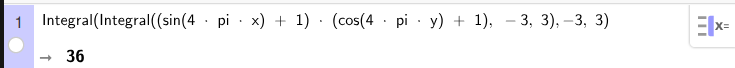
\includegraphics[width=0.8\textwidth]{./img/ggb_integral.png}
    \caption{積分正確答案-使用Geogebra計算}
\end{figure}
\begin{figure}[H]
    \centering
    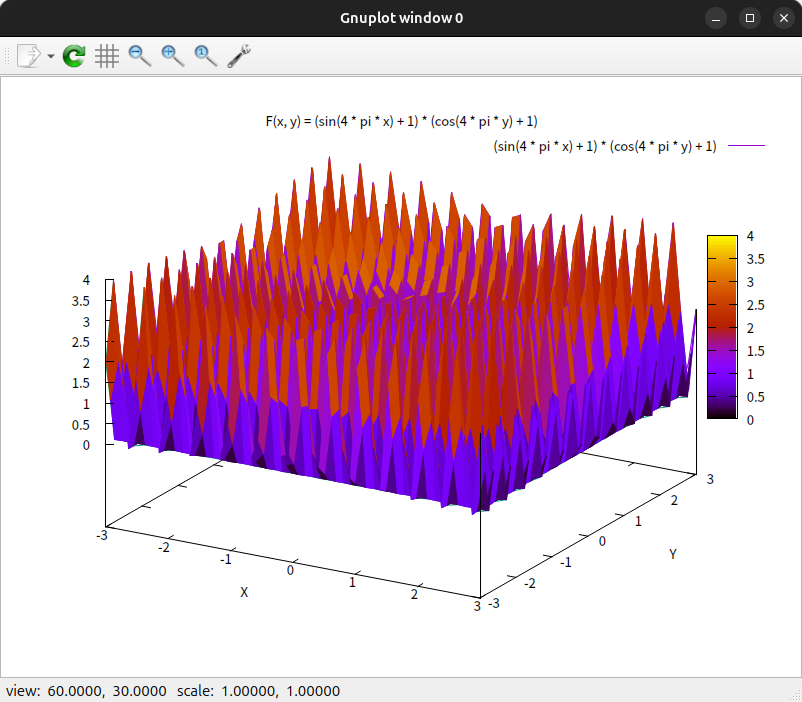
\includegraphics[width=0.8\textwidth]{./img/func_image.png}
    \caption{$f(x,y) = (sin(4 * pi * x) + 1) * (cos(4 * pi * y) + 1)$}
\end{figure}

\subsection{P-Refinement}
$N$為Legendre多項式次數,$Result$為積分值,$Error$為誤差。
\begin{longtable}{|c|c|c|c|c|c|c|c|}
    \hline
    N & Result & Error & N & Result & Error\\
    \hline
    2 & 9.1188491146e-01 & 3.5088115089e+01 & 18 & 1.8413133260e+01 & 1.7586866740e+01 \\
    \hline
    3 & 3.9999637870e+01 & 3.9996378703e+00 & 19 & 4.6208395774e+01 & 1.0208395774e+01 \\
    \hline
    4 & 6.4994893227e+01 & 2.8994893227e+01 & 20 & 3.1395581187e+01 & 4.6044188129e+00 \\
    \hline
    5 & 4.0440463347e+01 & 4.4404633474e+00 & 21 & 3.7696229819e+01 & 1.6962298190e+00 \\
    \hline
    6 & 2.8290249855e+01 & 7.7097501451e+00 & 22 & 3.5473701296e+01 & 5.2629870408e-01 \\
    \hline
    7 & 1.9756218686e+01 & 1.6243781314e+01 & 23 & 3.6140478205e+01 & 1.4047820528e-01 \\
    \hline
    8 & 5.4755662235e+01 & 1.8755662235e+01 & 24 & 3.5967235045e+01 & 3.2764954577e-02 \\
    \hline
    9 & 5.6083021904e+01 & 2.0083021904e+01 & 25 & 3.6006759412e+01 & 6.7594119433e-03 \\
    \hline
    10 & 4.6797642332e+01 & 1.0797642332e+01 & 26 & 3.5998754483e+01 & 1.2455171449e-03 \\
    \hline
    11 & 3.4682639395e+01 & 1.3173606046e+00 & 27 & 3.6000206651e+01 & 2.0665102727e-04 \\
    \hline
    12 & 2.4753251334e+01 & 1.1246748666e+01 & 28 & 3.5999968916e+01 & 3.1083542787e-05 \\
    \hline
    13 & 3.5058279612e+01 & 9.4172038778e-01 & 29 & 3.6000004264e+01 & 4.2635055522e-06 \\
    \hline
    14 & 5.0119759982e+01 & 1.4119759982e+01 & 30 & 3.5999999464e+01 & 5.3598760275e-07 \\
    \hline
    15 & 3.1362156500e+01 & 4.6378434996e+00 & 31 & 3.6000000062e+01 & 6.2035162784e-08 \\
    \hline
    16 & 2.2474694991e+01 & 1.3525305009e+01 & 32 & 3.5999999993e+01 & 6.6364975737e-09 \\
    \hline
    17 & 5.7341100010e+01 & 2.1341100010e+01 & 33 & 3.6000000001e+01 & 6.5857364007e-10 \\
    \hline    
\end{longtable}

\subsection{H-Refinement}
$G * G$為Grid數量,$Result$為積分值,$Error$為誤差,$N = 8$。
\begin{longtable}{|c|c|c|c|c|c|c|c|}
    \hline
    G & Result & Error & G & Result & Error\\
    \hline
    1 & 5.4755662235e+01 & 1.8755662235e+01 & 17 & 3.6000000000e+01 & 7.1054273576e-15 \\
    \hline
    2 & 1.0081204098e+01 & 2.5918795902e+01 & 18 & 3.6000000000e+01 & 1.4210854715e-14 \\
    \hline
    3 & 3.4499874630e+01 & 1.5001253702e+00 & 19 & 3.6000000000e+01 & 2.1316282073e-14 \\
    \hline
    4 & 3.6043462043e+01 & 4.3462043139e-02 & 20 & 3.6000000000e+01 & 0.0000000000e+00 \\
    \hline
    5 & 3.6000000000e+01 & 0.0000000000e+00 & 21 & 3.6000000000e+01 & 7.1054273576e-15 \\
    \hline
    6 & 3.5999864294e+01 & 1.3570560129e-04 & 22 & 3.6000000000e+01 & 4.9737991503e-14 \\
    \hline
    7 & 3.6000000000e+01 & 7.1054273576e-15 & 23 & 3.6000000000e+01 & 2.8421709430e-14 \\
    \hline
    8 & 3.6000000000e+01 & 2.8421709430e-14 & 24 & 3.6000000000e+01 & 4.9737991503e-14 \\
    \hline
    9 & 3.6000000000e+01 & 1.4210854715e-14 & 25 & 3.6000000000e+01 & 2.1316282073e-14 \\
    \hline
    10 & 3.6000000000e+01 & 1.4210854715e-14 & 26 & 3.6000000000e+01 & 3.5527136788e-14 \\
    \hline
    11 & 3.6000000000e+01 & 1.4210854715e-14 & 27 & 3.6000000000e+01 & 2.8421709430e-14 \\
    \hline
    12 & 3.6000000003e+01 & 3.1435547498e-09 & 28 & 3.6000000000e+01 & 7.1054273576e-15 \\
    \hline
    13 & 3.6000000000e+01 & 7.1054273576e-15 & 29 & 3.6000000000e+01 & 1.4210854715e-14 \\
    \hline
    14 & 3.6000000000e+01 & 7.1054273576e-15 & 30 & 3.6000000000e+01 & 7.1054273576e-15 \\
    \hline
    15 & 3.6000000000e+01 & 4.2632564146e-14 & 31 & 3.6000000000e+01 & 3.5527136788e-14 \\
    \hline
    16 & 3.6000000000e+01 & 9.9475983006e-14 & 32 & 3.6000000000e+01 & 1.2789769244e-13 \\
    \hline
\end{longtable}


\subsection{Refinement}
橫軸為網格數量,縱軸為N,表格內容為誤差值。
\begin{longtable}{|c|c|c|c|c|c|c|c|c|}
    \hline
    & 3 & 4 & 5 & 6 & 7 & 8 & 9 & 10\\
    \hline
    2 & 2.03e+01 & 2.40e+01 & 7.11e-15 & 3.18e+01 & 2.13e-14 & 1.42e-14 & 1.42e-14 & 1.42e-14 \\
    \hline
    3 & 3.05e+00 & 2.65e+01 & 2.84e-14 & 1.91e+01 & 3.55e-14 & 6.39e-14 & 1.42e-14 & 2.84e-14 \\
    \hline
    4 & 1.22e+01 & 2.67e+01 & 7.11e-15 & 4.53e+00 & 7.11e-15 & 4.26e-14 & 0.00e+00 & 2.13e-14 \\
    \hline
    5 & 2.88e+01 & 1.09e+01 & 7.11e-15 & 6.00e-01 & 7.11e-15 & 2.13e-14 & 7.11e-15 & 7.11e-15 \\
    \hline
    6 & 1.83e+01 & 2.56e+00 & 1.42e-14 & 5.12e-02 & 1.42e-14 & 7.11e-15 & 0.00e+00 & 2.84e-14 \\
    \hline
    7 & 6.45e+00 & 3.94e-01 & 7.11e-15 & 3.06e-03 & 1.42e-14 & 0.00e+00 & 2.13e-14 & 2.13e-14 \\
    \hline
    8 & 1.50e+00 & 4.35e-02 & 0.00e+00 & 1.36e-04 & 7.11e-15 & 2.84e-14 & 1.42e-14 & 1.42e-14 \\
    \hline
    9 & 2.52e-01 & 3.62e-03 & 7.11e-15 & 4.65e-06 & 1.42e-14 & 1.42e-14 & 7.11e-15 & 3.55e-14 \\
    \hline
    10 & 3.22e-02 & 2.36e-04 & 1.42e-14 & 1.27e-07 & 4.26e-14 & 1.42e-14 & 7.11e-15 & 4.26e-14 \\
    \hline
    11 & 3.26e-03 & 1.24e-05 & 0.00e+00 & 2.82e-09 & 4.26e-14 & 2.13e-14 & 7.11e-15 & 2.13e-14 \\
    \hline
    
\end{longtable}
\subsection{Visualize}
\begin{figure}[H]
    \centering
    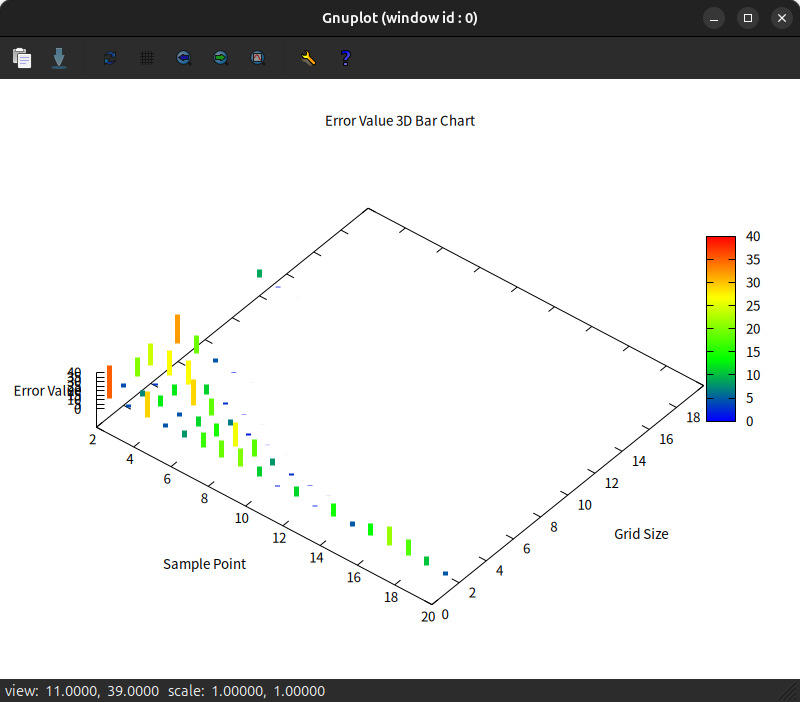
\includegraphics[width=0.8\textwidth]{./img/plot.png}
    \caption{Visualize}
\end{figure}

\section{心得}
這次作業實做了高斯積分,並透過網格量分段積分的方式(H-Refinement)和多項式次數的增加(P-Refinement)來進行誤差分析,最後透過Refinement來找比較哪個方法的誤差較小。\\
在實做過程中,原本是打算使用建表的方式來計算高斯積分的權重和採樣點,但在上網尋找資源時看到有人提供計算權重和採樣點的psuedo code,因此改用這個方法來計算,得到相比建表的方法更精確且彈性的結果。\\
在結果視覺化中,原本打算使用OpenGL,但後來想說嘗試看看使用gnuplot,因此最後使用gnuplot來繪製函數圖形以及誤差。

\section{參考資料}

\begin{thebibliography}{1}

\bibitem{pomax_legendre_gauss}
Pomax, “Gaussian Quadrature Weights and Abscissae”, \url{https://pomax.github.io/bezierinfo/legendre-gauss.html}

\end{thebibliography}

\end{document}

% xelatex  --max-print-line=10000 -synctex=1 -interaction=nonstopmode -file-line-error -recorder .\codebook.tex 